\section{Behavior}
\label{behavior}

The behavior of the icache interface is quite simple: to accept requests from the fetch stage and send them to the icache. To optimize and minimize the number of requests, it contains a buffer of 4 instructions, which correspond to the datablock of the cache. This is an architecture structure that needs to be invalidated in the case of a fence or exception to not affect the security of the core. 

There is some logic to manage the incoming requests and the buffer which is explained later in the state machine section.

\subsection{Exception}
In the current supported privilege ISA, the exceptions that can be originated from the Icache or icache interface are:
\begin{itemize}
	\item INSTRUCTION ACCES FAULT: Whenever it is used the first 24 bits of the PC since we only allow 40 bits addr. This is actually checked at the fetch stage.
	\item INSTRUCTION ADDR MISALIGNED is also checked at fetch stage.
	\item PAGE FAUL: it is reported by the icache interface.
\end{itemize}

\subsection{State Machine}

Figure \ref{fig:state_machine} shows the state machine that handles the logic of managing the icache requests. Some interactions are straight forward but for some other more information is given.

From \emph{ReqValid} or \emph{Replay} state to \emph{Noreq} state:
\begin{itemize}
	\item \textbf{req invalidate buffer:} is the condition when we want to invalidate the icache and or the buffer due to an exception or a fence.
	\item \textbf{Change addr Req:} is the condition when we change the request to the icache once it has already been sent another one previously. For example, we request the next pc but arrives a branch miss-prediction and needs to change the next pc. 
	\item \textbf{Resp Valid \& addr is != New request}: is the condition when we receive a response from the icache valid but the addr request has changed and is not equal to the response.
\end{itemize}

\begin{figure}[H]
	\centering
	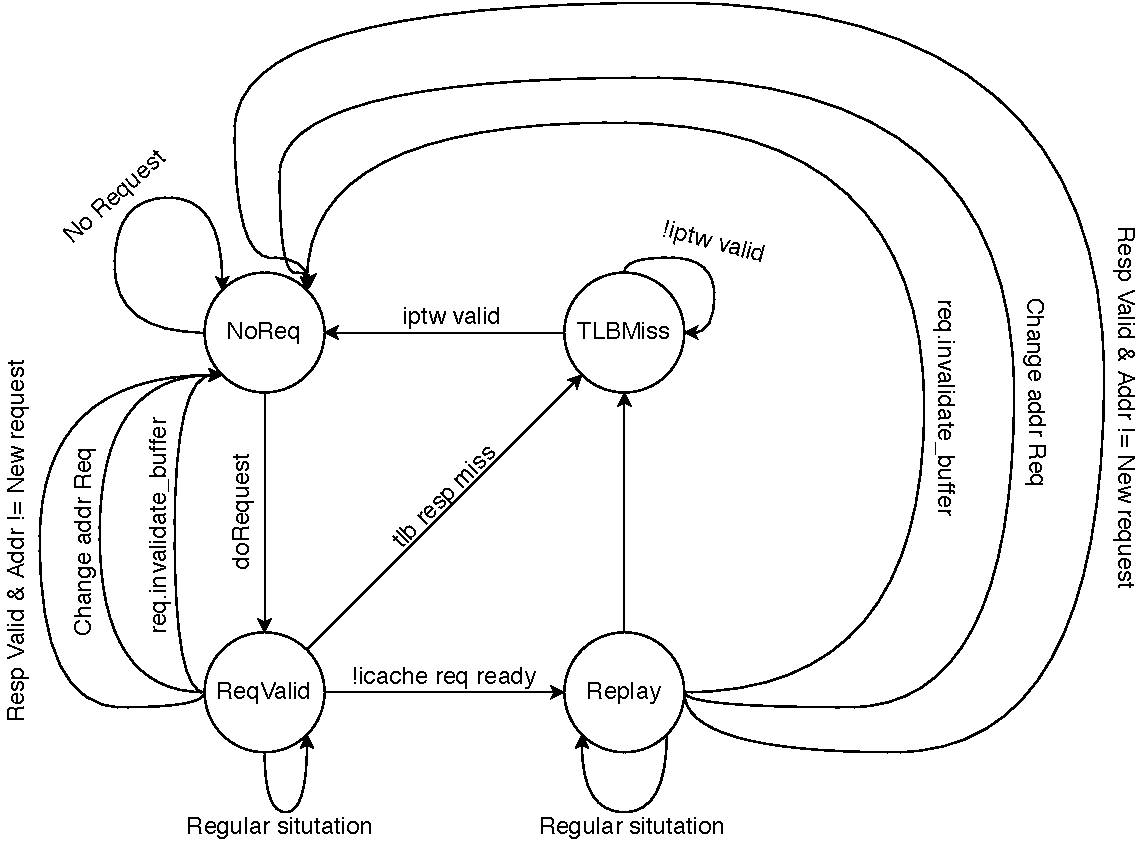
\includegraphics[width=\textwidth]{Figure/state_machine}
	\caption{Icache interface state machine}
	\label{fig:state_machine}
\end{figure}